% !TEX encoding = Windows Latin 1
\documentclass{llncs}
\usepackage{graphicx}
\usepackage[english]{babel}
\usepackage{color}
\usepackage{ucs}
\usepackage[latin1]{inputenc}

\newcommand{\markus}[1]{\textcolor{red}{Markus: #1}}
\newcommand{\arif}[1]{\textcolor{blue}{Arif: #1}}
\newcommand{\lars}[1]{\textcolor{greed}{Lars: #1}}

\renewcommand\floatpagefraction{.9}
\renewcommand\topfraction{.9}
\renewcommand\bottomfraction{.9}
\renewcommand\textfraction{.1}   
\setcounter{totalnumber}{50}
\setcounter{topnumber}{50}
\setcounter{bottomnumber}{50}

\bibliographystyle{splncs03}

\begin{document}
\frontmatter        
\pagestyle{headings}
\mainmatter           

\title{Model Fragmentation For High Access Performance of Models Persisted in Key-Value Stores}

\author{Markus Scheidgen}
\authorrunning{M. Scheidgen}
\institute{Department of Computer Science, Humboldt Universit�t zu Berlin\\
           Unter den Linden 6, 10099 Berlin, Germany\\
           \email{\{scheidge\}@informatik.hu-berlin.de}}

\maketitle
%\thispagestyle{empty}

\begin{abstract} 
\markus{TODO}
\end{abstract}

\section{Introduction}

Modeling frameworks (e.g. the Eclipse Modelling Framework (EMF) or kermeta) can only work with a model when it is fully loaded into a computer's main memory (RAM), even though not all model objects are used at the same time.
This limits the possible size of a model. 
Modeling frameworks themselves provide only limited capabilities to deal with large models (i.e. resources and resource lazy loading in EMF). 
Model persistence frameworks (e.g. Connected Data Objects (CDO)) on the other hand, store models in data bases and load and unload single model objects on demand. 
Only those objects that are used at the same time need to be maintained in main memory at the same time. This allows to work with models larger than the main memory otherwise allows. 

We claim that existing data base persistence solutions may provide a main memory efficient solution to the model size issue, but not a time efficient one. In this paper, time efficiency always relates the time it takes for a single execution of one of four abstract modeling tasks. These tasks are (1) creating and extending models, (2) traversing models (e.g. as necessary during model transformation), (3) querying models, and (4) loading parts of models (i.e. loading a diagram into an editor).

An obvious observation is that some of these modeling tasks (especially traversing models and loading parts of models) require to load large numbers of model objects eventually. Existing persistence frameworks, store and access model objects individually. If a tasks requires to load a larger part of the model, all its objects are still accessed individually from the underlying data base. This is time consuming.

Our hypothesis is that modeling tasks can be executed faster, if models are mapped to larger aggregates within an underlying data base. Storing models as aggregates of objects and not as single objects reduces the number of required data base accesses, or as Martin Fowler puts it on his blog: \emph{"Storing aggregates as fundamental units makes a lot of sense} [...]\emph{, since you have a large clump of data that you expect to be accessed together"},~\cite{martinFowler}. This hypothesis raises three major questions: Do models contain aggregates that are \emph{often} accessed together? How can we determine aggregates automatically and transparently? What actual influence on the performance has the choice of concrete aggregates?

To answer these question, we will proceed as follows: First (section~\ref{sec:applications}), we look at three typical modeling applications: which model sizes they work with and what concrete modeling tasks they perform predominantly. This will give us an idea of what aggregates could be and how often aggregates can be expected to be actually accessed together. 
Secondly (section~\ref{sec:fragmentation}), we will present our approach to finding aggregates within models. This approach is based on fragmenting models along their containment hierarchy (a fix inherent spanning tree that exist in each model). We will reason, that most modeling tasks need to access aggregates that are sub-trees of the containment hierarchy (fragments). 
In the related work section~\ref{sec:related_work}, we present existing model persistence frameworks and interpret their strategies with respect to the idea of fragmentation. Furthermore, we discuss key-value stores for persisting fragmented models.
The following section provides a theoretical analysis and upper bound estimation for possible performance gains of optimal fragmentation.
In section~\ref{sec:implemention}, we finally present a framework that implements our fragmentation concept.
The next section is the evaluation section: we compare our framework to existing persistence frameworks with respect to time and memory efficient execution of the four abstract modeling tasks. Furthermore, we use our framework to measure the influence of fragmentation on performance to verify the analytical considerations from section~\ref{sec:fragmentation}.
We close the paper with conclusions and further work. 


\section{Related Work}
\label{sec:related_work}

\subsection{Model Persistence}
For EMF based models, there are at least four different approaches to large models: (1) regular EMF with XMI based persistence; (2) EMF resources, where a resource can be a file or an entry in a data base; (3) CDO~\cite{cdo} and other object relational mappings (ORM) for Ecore; (4) morsa~\cite{morsa2011} a EMF data-base mapping for non-relational data bases.
\footnote{Mentioned memory and time efficiency in this section are taken from the evaluation section~\ref{sec:evaluation}.}

First, regular EMF: Models are persisted as XMI documents and can only be used if loaded completely into a computer's RAM. EMF realises the \emph{no fragmentation} strategy. The memory usage of EMF is linear to the model's size. It's time efficiency is good for small models, since it needs no further managing overhead, but is bad for large models due to pointless garbage collection and extensive allocation of memory.

Secondly, EMF resources~\cite{emf2009}: EMF allows to fragment a model into different resources. Originally, each resource could only contain a separate containment hierarchy and only cross-references were allowed. But since EMF version 2.2 containment proxies are supported. EMF support lazy loading: resources do not have to be loaded manually, EMF loads them transparently once the first object of a resource is accessed. Model objects have to be assigned to resources manually (\emph{manual fragmentation}). To actually save memory the user has to unload resources manually too. Memory efficiency is good if resources are handled properly. Time efficiency is also good due to minimal management overhead. The framework MongoEMF~\cite{mongoEMF} maps resources to entries in a MongoDB~\cite{mongodb2010} data base.

Thirdly, CDO~\cite{cdo}: CDO is a ORM for EMF.~\footnote{Lately, CDO also support non-relational data bases, such as MongoDB~\cite{mongodb2010}. Such features were not evaluated in this paper; but one can assume characteristics similar to those of morsa.}
It supports several relational data bases. Classes and features are mapped to tables and their columns. Objects, references, and attributes are mapped to rows. CDO was designed for software modeling and versioning and provides transaction, views, and versions. These features produce some overhead. 
Relational data bases and SQL provide mechanisms to index and access objects and their features. This allows fast queries, if the user understands the underlying ORM. But, complex table structures and indexes cause very low entry (i.e. object) creation rates. Sorting entries into indexes and tables consumes time.
CDO is RAM efficient. Traversing or loading parts of models is slow, because each object needs to be accessed individually. 

Fourthly, morsa~\cite{morsa2011}: Different to CDO, morsa uses so mongoDB~\cite{mongodb2010}, a no-sql data base. In no-sql data bases (or other key-value stores) store arbitrary values in an key-value map. This simple data structure allows fast and easy distributable data bases. Morsa stores objects, their references and attributes as JSON documents. Morsa furthermore uses mongoDB's index feature to index specific characteristics (e.g. an objects meta-class reference). This produces similar characteristics than with CDO: fast queries, slow creation, traverse, and load.

\subsection{Key-Value Stores}

The general term \emph{data base} has long been used as a synonym for relational data bases. But in the last decade a new kind of data base has become more and more popular. Web and cloud computing require scalability above all, and traditional ACID~\cite{ACID} properties can be sacrificed if the data store is easily distributable. This explains the popularity of so called \emph{No-SQL} data bases or \emph{key-value store}. Such key-value stores only provide a simple map data structure: there are only keys and values. For more information and an comparison of existing key-value stores refer to~\cite{nosql2010}.

Key-value stores are ideal data bases for persisting fragmented models. Fragments can be identified by URIs, which are easily mapped to key-value store keys, and XMI (as native model persistence format) can be used for values. Key-value stores provide a scalable persistent solution with good performance characteristics. This allows to react to increasing requirements for model sizes and number of parallel access (e.g. for the geo-spatial models modelling application).

There are three different applications that inspired three groups of key-value stores. First, there are web applications and the popular MongoDB~\cite{mongodb2010} and CouchDB~\cite{couchdb2010} data bases. These use JSON documents as values and provide additional indexing for JSON attributes.

Secondly, there is cloud computing and commercial Google Big-Table~\cite{bibtable2006} and Amazon's Dynamo~\cite{dynamo2007} inspired data stores. HBase~\cite{hbase2008} and Cassandra~\cite{cassandra2009} are respective open source implementations. Those data bases strive for massive distribution, they provide no support for additional value structuring, but integrate well into map-reduce~\cite{mapreduce} execution frameworks, such as Hadoop (HBase is Hadoop's native data store). 

A third application is high performance computing. Scalaris~\cite{ScalarisTransactions2008} is a key-value store opt for massive parallel, cluster, and grid computing. Scalaris provides mechanisms for consistency and transactions and brings some ACID to key-value stores.

For the implementations in this paper, we use HBase, which provides everything we need and nothing more.
\section{Examples for (Extra) Large Models}

\subsection{Software Projects -- e.g. Linux Kernel}

\subsubsection{What are software code models?}
We use the term model to describe MDSD artifacts. Originally these artifacts were models on a high level of abstraction, but today programming code, can also be understood as models. For example IDEs such as eclipse JDT or eclipse CDT internally maintain programming code as ASTs (primitive models) in order to provide advanced IDE features such as outlines, error annotations, type and call hierarchies, and code completion. It is safe to assume that programming code contains far more information compared to high-level models. Since we are looking for extra large models, we will concentrate on software code models.

Advances in language workbenches suggest to replace these IDEs with eclipse EMF based and generated tools. Advances in comparison and versioning of models will soon allow to replace per-line-text-file-based versioning systems (e.g. CSV, SVN, GIT) with model based (e.g. EMF-based) systems that version on a per mode-object- or even per-object-attribute basis.

\subsubsection{How big is are existing software code models?}
How large are these software code models? Traditionally code size is measured in \emph{lines of code} LOC (physical lines), SLOC (source LOC, like LOC but without empty lines, comments, duplicates; refer to Wheeler~\cite{wheeler}, and LLOC (logical LOC, like SLOC but normalized to one statement per line). These measures exist for many known software projects (and their history) and can be easily captured for open source projects. 

In order to determine corresponding model sizes, we need to know how much model objects each LOC represents. To estimate this, we used the eclipse CDT parser as tool and the linux kernel as sample. The CDT parser is specialized to parse C/C++ code in its un-preprocessed form. Thus, the resulting ASTs are not bloated with information injected (with lots of duplicates) during pre-processing. Of course ASTs are not software models as they are understood in the OMG/EMF world, but we can assume that proper C/C++ models will contain one object for each AST node. \markus{This needs a reference}. Parsing the current kernel version, counting its AST nodes, and comparing this number to the kernel's SLOC number gives us a good estimate for objects per SLOC (at least for the kernel code, probably for all C code, and maybe it is also a good estimate for other similar programming languages, e.g. C\#, Java). We will use this estimate to extrapolate the model size of other kernel versions and other software projects. 

Eventually, we want to store software models and its versions. Of course, we only want to store the differences between versions. A software projects model size is determined by the size of the differences that produced the current software model. To determine this size, we need to know how much LOCs were added, removed, and modified in a software project. To estimate this, we use the versioning system GIT as tool and the linux kernel GIT repository as sample. With gitstats we can determine the number of added, removed, and changed lines throughout the repository history. With these numbers, the estimated objects per SLOC and the recorded SLOCs for different kernel versions we can estimate the model size of a kernel software code model repository. We can also assume that other software projects have a similar proportion of added, removed, and modified lines, and transfer these estimates to other software projects. 

\begin{figure}
  \centering
  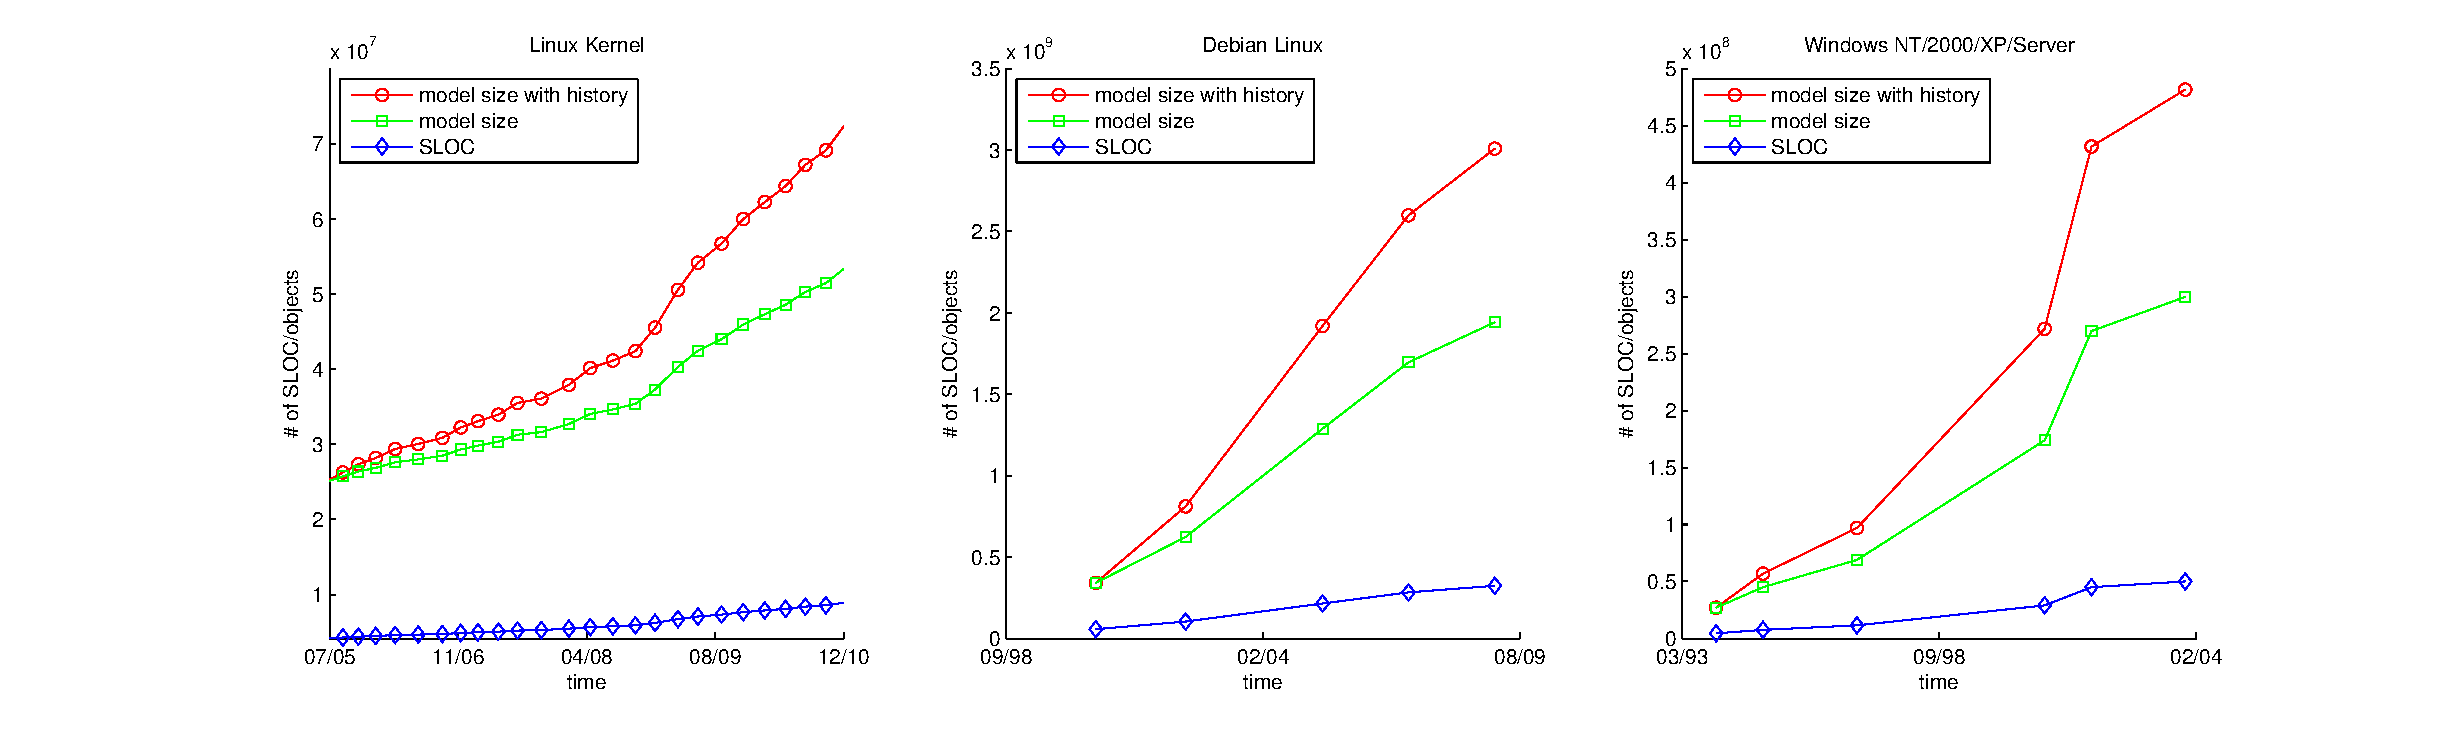
\includegraphics[width=\linewidth]{figures/software_model_sizes}
  \caption{SLOC and estimated number of objects for popular large software projects.}
  \label{fig:software_model_sizes}
\end{figure}

Fig.~\ref{fig:software_model_sizes} shows the LOC numbers and estimated object numbers in corresponding software code models. The charts present different software projects and how size developed over time. \markus{kernel, linux(debian)?, windows - numbers based on kernel git alone, SLOC numbers and transferred kernel estimates.}

\subsubsection{How big are software code models in the future?}

Some believe that the average size software (and software code models for that matter) grows faster than linear following Moore's Law. Maciej Soltysiak for example has analysed the grows of the linux kernel code base and observed exponential growth. A counter argument is that software not only bound by hardware limitations (i.e. Moore's Law) but increasingly by software complexity and therefore will not grow exponentially. Never the less, it is safe to assume that software code models will be larger in the future.


\subsection{Geospatial Models -- e.g. a 3D Model of Berlin in CityML}

\subsubsection{What are geo-spatial 3D city models?}
3D city models are a good example for structured desecrate geo spatial information. In these models geo spatial features like windows, rooms, apartments, houses, streets, boroughs, and cities are composed to form a complex graph. The CityGML standard, provides a set of xml-schemas (building upon other standards, e.g. GML) that function as a meta-model. CityGML, compared to other quasi standards (e.g. google KML) does not solely concentrate on the 3D measures, but allows to extend the covered information by more semantic attributes (e.g. materials, age, inhabitants, existing infrastructure, etc.). Geo spatial models usually come with different levels of details (LOD); CityGML distinguished 5 LODs, 0-4). 

\subsubsection{How big is an existing 3D city model?}
Like many cities, Berlin is currently establishing such a model. The current model of Berlin comprises all of Berlin, but mostly on a low-medium level of detail (LOD 1-2). To get an approximation of the model's size, we counted the XML entities. The current Berlin model, contains roughly $128*10^6$ objects. 

\subsubsection{How big will 3D city models get in the future?}
Based on data published in~\cite{CityGMLBerlinDB} a LOD 1 building comprised of 12.5 objects, a LOD 2 building of 40 objects, a LOD 3 building of 350 objects. A LOD 3-4 building of Berlin would therefore consist of $1*10^9$ objects. Berlin inhabits 3.5 million people. About 50\% of the worlds $7*10^9$ people live in cities. This gives a whole LOD3-4 approximation of $10^{12}$ objects for a \emph{world 3D city model}.

\subsection{Heterogenous Sensor Data -- e.g. HWL and Smart City}

\subsubsection{What are sensor data models?}
Sensor data usually comprises of time series of measured physical values in the environment of a sensor; but sensor data can also contain patterns of values (e.g. video images). Sensor data is collected in sensor networks, that combine distributes sensors with an communication infrastructure. Sensor data can be heterogenous: a sensor network can use different types of sensors that measure a multitude of parameters. 
\markus{cites, cites, cites}. 

We build the \emph{Humboldt Wireless Lab} are 120 node wireless sensor network. Nodes are equipped with 3 axis accelerometer, but more essentially for our research also creates data from monitoring all running software components. Components provide data as structured XML documents. Software components are themselves structures according to the software architecture.

We build a software that collects this XML data, transforms it into an EMF model, stores it in a database, and allows analysis with EMFs generated Java APIs and model transformation languages (e.g.~\cite{SMTLpaper}).

\subsubsection{How big are existing sensor data models?}
Network protocol and system software components provide 372 distinct data sets (containing data such as WLAN radio data, network statistics, CPU load levels, etc.) Each data set is represented in an XML fragment of variable size. Per second each node in the network produces XML entities that translate into an average of 1120 EMF objects. A common experiment with HWL involves 50 nodes and measures of a period of 24h. Such an experiment produces $5*10^9$ objects. 

\subsubsection{How big can sensor data models get in the future?}
Sensor networks are currently only limited by the limitations of the technical infrastructure that supports them. Will, infrastructure, and money provided, sensor networks can produce models of virtually unlimited size. 


\section{Possible performance gains for loading models from local key-value data stores}

In this section, we analyse the performance gains from optimal model fragmentation. Even though these gains will never be achievable for real applications (in most cases), the results in this section provide a theoretical lower bound. The results also help to benchmark (existing) fragmentation strategies. 

\subsection{Optimal Fragmentation for non Distributed and Unordered Data Stores}

First, we need to define a few functions that provide the performance of all operations involved in loading a model. We define the \emph{local load} function $ll$ that determines how long it takes to load a model of a given $size$  from a local data store:

$$ll:size\rightarrow t=\mathcal{O}\left(size\right)$$

The next function \emph{find entry local} $fl$ determines how long it takes to find an entry in a local key-value data store based on the number of key $\#keys$, i.e. number of entries:

$$fl:\#keys\rightarrow t=\mathcal{O}log(\#keys)$$

We will use the following parameters: The total model $size$, the average number of objects per entry $ope$, the size of the model to load $load$, and $part$ the average percentage of an entry's objects that belong to the loaded model if at least one object is part of the loaded model.

The time $t$ to load a model with this parameters is:

\begin{eqnarray*}
t&=&\frac{load}{part*ope}\left(fl(\frac{size}{ope}) + ll(ope)\right)\\
&=&\mathcal{O}\frac{load}{part*ope}\left(log(\frac{size}{ope})+ope\right)\\
\end{eqnarray*}

The two extreme examples are: (only one big entry) $ope=size$, $part=load/size$, $t=\mathcal{O}\left(size\right)$, and (one object per entry) $ope=1$, $part=1$, $t=\mathcal{O}\left(load\left(log(size)+1\right)\right)$. 

\subsubsection{Analysis}
In the optimal model distribution (one only wants to load models that exactly constitute one entry) $ope=load$ and $part=1$ the time is $t=\mathcal{O}\left(log(\frac{size}{load})+load\right)$.

\begin{figure}
  \centering
  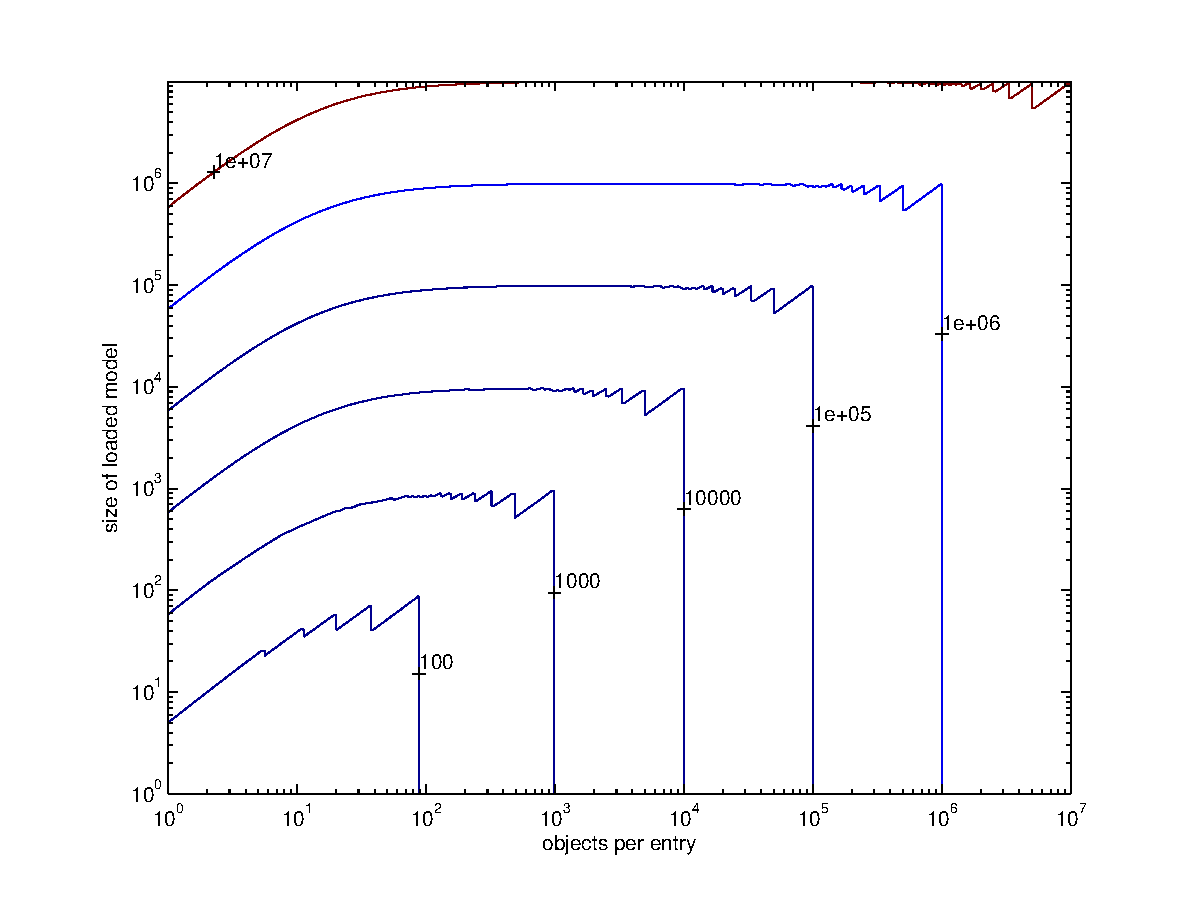
\includegraphics[width=0.65\linewidth]{figures/optimal_load_times}
  \caption{Load times}
  \label{fig:optimal_load_times}
\end{figure}

The plot in Fig.~\ref{fig:optimal_load_times} shows the relation between objects per entry, load size, and the time it takes to load. The contours show loads that take the same time. The plot does not account for any $ll=m*size+n$ and $fl=m*log(\#keys)+n$ factors ($m,n$). Depending on actual factors (see next section) the linear or logarithmic parts of the contours are more or less dominant. If parsing is relatively slow, fragmentation becomes more important (linear parts of contours are longer), if accessing the data-base becomes relatively slow, fragmentation becomes less relevant and generally large object per entry numbers are more desirable (logarithmic parts of contours are longer).

\subsubsection{Measurements}

We measured the performance of EMF parsing (depending on model size) and HBase data store access (depending on number of data store entries). The results are shown in Fig.~\ref{fig:optimal_load_times}. As expected the parsing performance is linear and the data store access behaves logarithmic. The plot in Fig.~\ref{fig:optimal_load_times_measured} is similar to Fig.~\ref{fig:optimal_load_times}, but uses $ll$ and $fl$ factors based on the measurements (actually the interpolated functions shown as lines in the plots).  

From this plot, we can see what fragmentation allows compared to no fragmentation ($ope=size$) or complete fragmentation ($ope=1$). No fragmentation always takes the full time (10s in this scenario). Of course optimal results can be obtained if ($load=ope$). This optimal result allows to load models a 1000 times bigger at the same time than total fragmentation. 

\begin{figure}[ht]
\begin{minipage}[b]{0.5\linewidth}
\centering
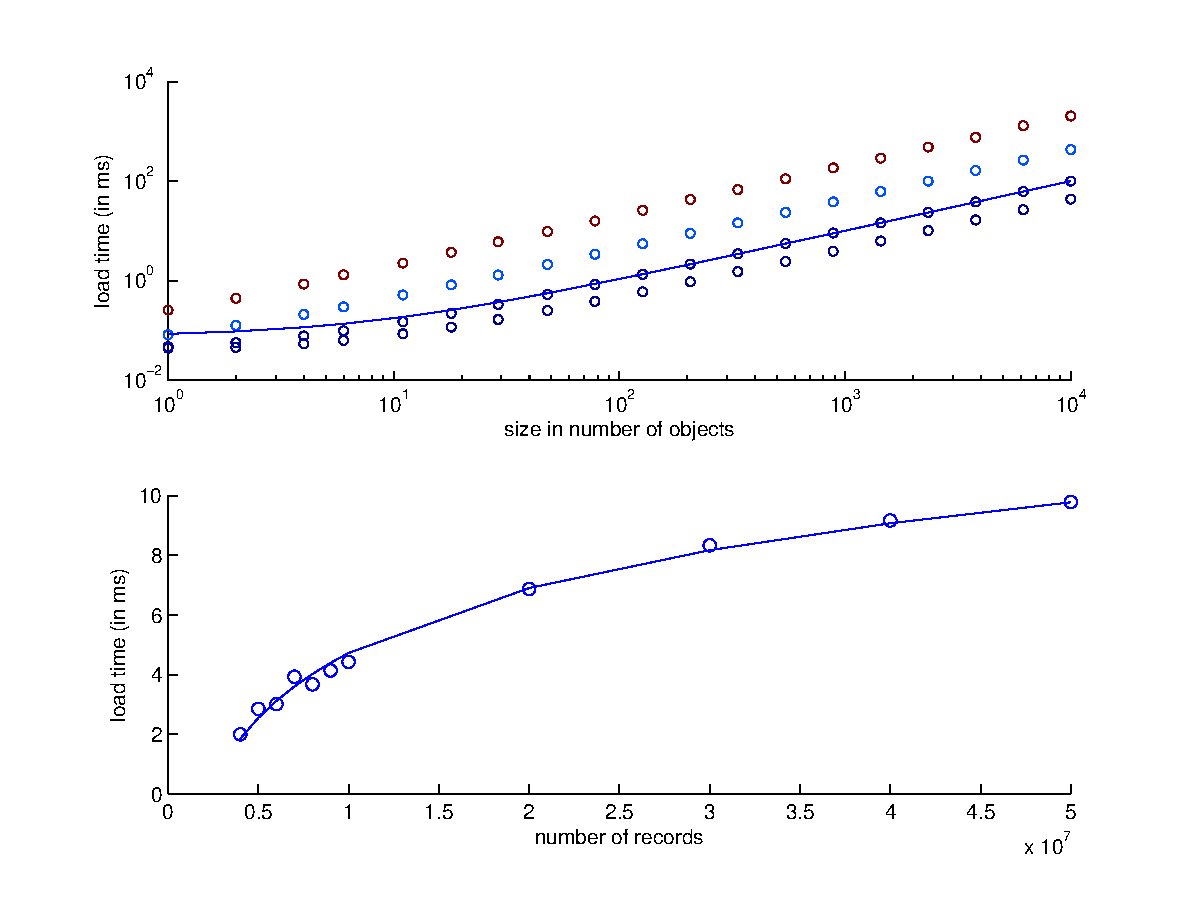
\includegraphics[width=\linewidth]{figures/emf_hbase_performance_measured}
\caption{Measure for liner parsing performance of EMF and logarithmic access performance of HBase.}
\label{fig:figures/emf_hbase_performance_measured}
\end{minipage}
\hspace{0.5cm}
\begin{minipage}[b]{0.5\linewidth}
\centering
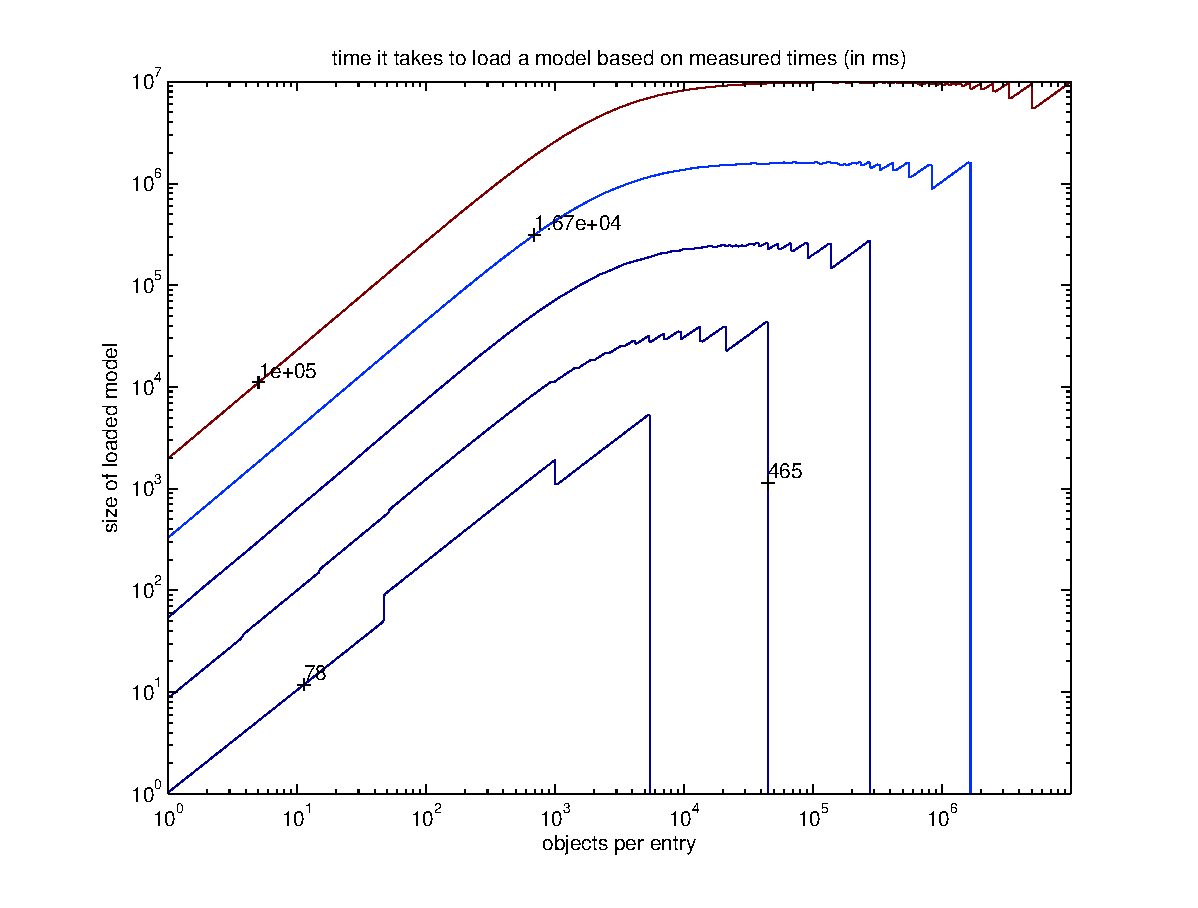
\includegraphics[width=\linewidth]{figures/optimal_load_times_measured}
\caption{Load times based on actual EMF parsing and HBase access measurements.}
\label{fig:optimal_load_times_measured}
\end{minipage}
\end{figure}

\subsection{Optimal Fragmentation in Ordered but Non Distributed Stores}

In ordered stores, entries can be scanned. If keys are chosen intelligently, a loaded model consisting of multiple fragments can still be with only one logarithmic access and subsequent scans. Assuming that all keys are always chosen in the optimal way and that the time between scans is close to 0: as long as $ope<load$ the required load time equals $ll(load)$. We can have more fine grain fragmentation without loosing performance if larger models are loaded. 

\subsection{Optimal Fragmentation in Unordered but Distributed Stores}

\section{Fragmentation Strategies}

\subsection{Manual Fragmentation}
\subsection{Metamodel Defined Fragmentation}

\begin{figure}[ht]
\begin{minipage}[b]{0.5\linewidth}
\centering
\includegraphics[width=\linewidth]{figures/metamodel_fragmentation_patterns_tree}
\caption{An example pattern in a model and a fragmentation. The red links are inter fragment links.}
\label{fig:metamodel_fragmentation_pattern_tree}
\end{minipage}
\hspace{0.5cm}
\begin{minipage}[b]{0.5\linewidth}
\centering
\includegraphics[width=\linewidth]{figures/metamodel_fragmentation_patterns_graph}
\caption{Another example pattern. For a single feature there are two types of instances: inter- and intra-fragment links.}
\label{fig:metamodel_fragmentation_pattern_graph}
\end{minipage}
\end{figure}

\subsubsection{Theory}
Access patterns for a model are strongly influenced by its metamodel.
Metamodels are tiny in comparison to their large instances. 
If you imagine looking from above onto a large model, the metamodel types of its objects form patterns. How we access a model is also influenced by its metamodel, since all algorithms doing something with a model are programmed against its metamodel.
Hence, optimal fragmentation goes along this patterns.
Most fragments will have the same structure, and fragments are connected through structural features of only few different types.
One way to define fragmentation is to mark these fragment crossing structural features. 

Fig.~\ref{fig:metamodel_fragmentation_pattern_tree} shows a simple example metamodel type pattern. The instances (links) of feature \emph{a} cross fragment borders (inter fragment links). All other links are intra-fragment links. The situation is a  little more complicated in Fig.~\ref{fig:metamodel_fragmentation_pattern_graph}. Here the links of feature \emph{c} have both inter- and intra-fragment instances. 

If we want to describe fragmentation by marking features as inter- or intra-fragment features, it would work for the example in Fig.~\ref{fig:metamodel_fragmentation_pattern_tree}, but not for the example in Fig.~\ref{fig:metamodel_fragmentation_pattern_graph}. Obviously, we need further restrictions.

Models (as used in this paper) always have a inherent spanning tree. The spanning tree is formed from links that are instances from containment features. All instances of containment features are part of the spanning tree. If we only allow containment features to be inter-fragment features then the instances of inter-fragment feature will always define a unique fragmentation. \markus{Proof?}

\subsubsection{Implementation}
This describes an implementation based on EMF. 

\subsection{Automated Fragmentation based on Expected Range Queries}
\subsection{Automated Fragmentation based on Access Patterns}
\subsection{Fragmentation of Even Models}

\subsubsection{Analysis}

At the beginning, we will look at \emph{even} models. A model is even, if its inner structure suggest fragmentation into equal pieces. For example, an intuitive way to fragment a OO software model is to put each package into one entry. This is an uneven model, since packages have different sizes. Another example is sensor data, sensor data produced at each point in time or on each node has the same size. If one puts each sensor reading or each node into one entry, the entries will have similar size.

Previously, we were looking the gains achieved with optimal fragmentation. While optimal fragmentation is plausible in manually fragmented models for a single specific loaded model (e.g. accessing single sensor readings in ClickWatch). Optimal fragmentation is unlikely for different loaded models (even impossible for models of different size). 

In general, we can assume that the smaller $ope$ is compared to $load$, the more likely it is that much of each entry is part of the loaded model. In other words, the smaller my entries are, the more likely it is that much or all if a single entry is part of the loaded model. We will model $part$  accordingly.
\section{Evaluation}

\subsection{Grabats -- An Actual Software Model}

\begin{figure}
  \centering
  \includegraphics[width=0.65\linewidth]{figures/grabatsLoadTraverse}
  \caption{Execution time for a full model traversal}
\end{figure}

\begin{figure}
  \centering
  \includegraphics[width=0.65\linewidth]{figures/grabatsLoadTraverseMem}
  \caption{Memory usage for a full model traversal}
\end{figure}

\begin{figure}
  \centering
  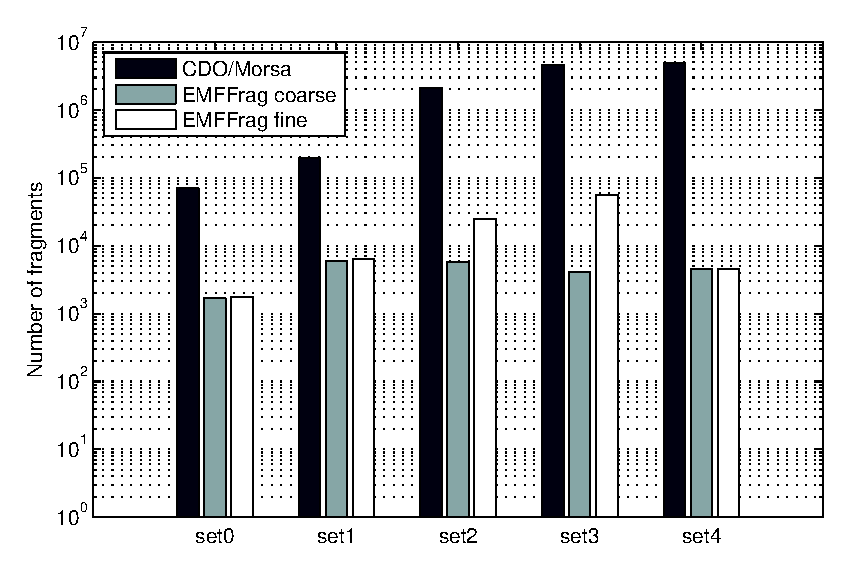
\includegraphics[width=0.65\linewidth]{figures/grabatsFragments}
  \caption{Number of fragments used}
\end{figure}

\begin{figure}
  \centering
  \includegraphics[width=0.65\linewidth]{figures/grabatsQuery}
  \caption{Execution time for a specific query}
\end{figure}
\section{Future Work} 
\label{future_work}

\subsubsection{Sorted and Distributed Key-Value Stores} 

Our fragmentation strategy is based on unsorted key-value store accesses with $\mathcal{O}log$ complexity. Neither our analysis, nor out  implementation EMFFrag, or our evaluation consider sorted key-value stores that allow to access sequential keys with constant time (scans). Neither did we consider distributed key-value stores which would allow parallel access. Key-value stores are easily distributed in peer two peer networks. This is done for two scalability reasons: replication (allows more users to access the same data in less time) and sharding (distributing data to allow faster and larger storage). Fragmentation can have an influence on both.

\subsubsection{Transactions}

If multiple user access/modify transactions become a necessity. Transaction can either be provided by the underlying data store (e.g. with Scalaris~\cite{ScalarisTransactions2008}) or can be implemented into EMFFrag. On non-distributed data stores, a common transaction pattern could be used. More interesting is explore the influence of fragmentation on transactions (and versioning), because the maximum granularity is determined by fragment size.

\subsubsection{Cross-References} 

EMFFrag persists containment references with URIs with a fragment ID pointing to the fragment that contains the reference objects. This does not work for cross references: when an object is moved, its URI changes and all referencing object use invalid URIs. For this reason EMFFrag needs to use a secondary index that maps object IDs to containing fragments. EMFFrag uses URIs with object IDs to persist cross references. To resolve such an URI, the secondary index is used to find the fragment that contains the object. Object IDs and secondary index are only maintained for objects that are actually cross references to keep the index small. 

In our analysis and evaluation, we did not examine the influence of cross references and corresponding indexes on performance. We have to expect that create/modify tasks are performed considerably slower, since two indexes have to be maintained. The impact on traverse, query, or partial loads, on the other hand, should be minimal.

\subsubsection{Large Value Sets}

In large models, single objects can become very large themselves if they hold large sets of attribute values and references. CDO maps an object's feature values to individual entries in a database table and can manage such objects, but does so slowly. EMFFrag (and Morsa), on the other hand, consider objects as atomic entities and large object become a performance burden too. We need to extend the fragmentation idea to large value sets. Similar to all consideration in this paper, these strategies for large value sets have to be optimized and evaluated for the abstract tasks manipulation, iteration (traverse), indexed access (query), and range queries (partial load). 

\section{Conclusions}\label{sec:conclusions}

Large software models consist of upto $10^9$ objects. Models from other application can have a size upto $10^{12}$ objects. Traversing models and loading larger aggregates of objects are common tasks (section~\ref{sec:applications}). Depending on fragment size, partially loading models can be done faster than loading whole models or loading models object by object. There is no optimal fragment size, but intermediate fragment sizes provide a good approximation  (sections~\ref{sec:gains} and~\ref{sec:evaluation}). We provide a persistence framework that allows automatic and transparent fragmentation, if appropriate containment features are marked as fragmentation points in the meta-model (sections~\ref{sec:fragmentation} and~\ref{sec:implemention}). We compared our framework to existing frameworks (EMF XMI, CDO and Morsa) and our framework performs significantly better for creating/manipulating, traversing, and partially loading models. Execution times are 5 to 10 times smaller. Model queries (that favour object-by-object based model persistence with indexes, such as in CDO and Morsa) can be executed with comparable execution times (section~\ref{sec:evaluation}). Model fragmentation also determines the granularity of transactions, which can be a disadvantage. Further problems are single objects with features that can hold large value sets; the fragmentation approach has to be extended for fragmentation of such value sets (section~\ref{sec:future_work}). Our framework stores fragments in key-value stores. Those scale easily (both replication and sharding is supported) and integrate well in peer-to-peer computation scheme (e.g. map-reduce). Fragmentation therefore prepares very large models for modelling in the cloud applications (section~\ref{sec:related_work}).

\bibliography{bibliography}

\end{document}
